% concatenated from main_arxiv.tex, table_field1.tex, table_field2.tex
\documentclass[a4paper,11pt]{article}
\usepackage[utf8]{inputenc}
\usepackage[english]{babel}
\usepackage{expl3}
\usepackage{amsmath,amssymb,amsfonts,amsthm,mathtools,bm}
\usepackage{siunitx}
\usepackage{booktabs}
\usepackage{microtype}
\usepackage{xcolor}
\usepackage{graphicx}
\usepackage{tikz}
\usetikzlibrary{arrows.meta,positioning}
\definecolor{cobalt}{RGB}{0,71,171}
\usepackage[colorlinks,urlcolor=cobalt,citecolor=cobalt,linkcolor=cobalt,
  pdfauthor={Sebastian Schaffer and Lukas Exl}]{hyperref}
\usepackage[nameinlink,noabbrev]{cleveref}
\usepackage{enumitem}
%\biboptions{numbers,sort&compress}
%\hfuzz=3pt

\usepackage{fullpage}

\usepackage{authblk}

\usepackage{url}

\newtheorem{proposition}{Proposition}
\newtheorem{remark}{Remark}
\newcommand{\R}{\mathbb{R}}
\newcommand{\m}{\bm m}
\newcommand{\z}{\bm z}
\newcommand{\p}{\bm p}
\newcommand{\s}{\bm s}
\newcommand{\Jop}{\bm J}
\newcommand{\Rop}{\bm R}
\newcommand{\Kop}{\bm K}
\newcommand{\Eenc}{E_{\theta}}
\newcommand{\Ddec}{D_{\xi}}
\newcommand{\Genergy}{g_{\eta}}
\newcommand{\zhat}{\widehat{\bm z}}
\DeclarePairedDelimiter{\norm}{\lVert}{\rVert}

\newcommand{\todo}[1]{\textcolor{red}{#1}}
\newcommand{\rmk}[1]{\textcolor{blue}{#1}}
\newcommand*\luk[2]{#2}
\newcommand*\change[2]{{\color{purple}{#2}}}

% Remove indentation globally
\setlength{\parindent}{0pt}

\setlength{\parskip}{5pt}

\begin{document}
\date{}
\title{An Energy-Based Conservative--Dissipative Latent Neural Evolution Operator for Magnetization Dynamics}

\author[a,b]{Sebastian Schaffer \thanks{\texttt{sebastian.schaffer@univie.ac.at}}}
\author[a,b]{Lukas Exl \thanks{\texttt{lukas.exl@univie.ac.at}}}

\affil[a]{Math. AI/ML, Wolfgang Pauli Institute, Vienna, Austria}
\affil[b]{Department of Mathematics, University of Vienna, Vienna, Austria}

\setcounter{Maxaffil}{0}
\renewcommand\Affilfont{\itshape\small}

\maketitle
\textbf{Abstract.} 
We develop an energy-based reduced-order model for micromagnetic magnetization dynamics that couples a convolutional autoencoder to a structured latent neural ordinary differential equation. Motivated by the precessional–dissipative structure of the Landau–Lifshitz–Gilbert equation, the latent vector field is generated from the gradient of a learned scalar potential through an antisymmetric operator and a symmetric positive-semidefinite dissipative operator. This potential is learned in nonunique latent coordinates and is not identified with the Gibbs free energy, but decreases monotonically along autonomous continuous-time solutions, while the antisymmetric component permits motion along its level sets. The encoder, decoder, latent energy, and operators are trained jointly on short trajectory windows using latent and decoded-rollout losses alone, without time-derivative supervision, physical-energy labels, or dissipation penalties. At inference, an initial state is encoded once, evolved in latent space, and decoded only at the requested output times, enabling substantially cheaper trajectory prediction than the micromagnetic solver used to generate the training data. We compare quadratic, deep, and additive deep–quadratic latent energies on two datasets parameterized by field amplitude and generated for the two applied-field directions of the NIST $\mu$MAG Standard Problem 4. Dissipative-only and antisymmetric–dissipative models achieve comparable accuracy on short training-style windows but differ substantially on uninterrupted rollouts, for which the antisymmetric–dissipative models provide markedly more accurate trajectory predictions. The deep–quadratic energy gives the best overall accuracy for both field directions and exhibits slower error growth when rollouts are extended to twice the training horizon.

\textbf{Keywords.} micromagnetics, energy-based model, reduced-order model, neural ordinary differential equation, latent dynamic

\section{Introduction}
Computational micromagnetics is widely used for the analysis and design of magnetic devices, including permanent magnets and integrated magnetic sensors \cite{brown1963micromagnetics,suess2018topologically,bashir2012head,fischbacher2018micromagnetics,kovacs2020computational}.
Their magnetization dynamics are commonly described by variants of the the nonlinear Landau--Lifshitz--Gilbert (LLG) equation \cite{gilbert2004phenomenological} or the Landau--Lifshitz equation
\begin{equation}
 \partial_t\m=-c_\gamma[\m\times\bm H_{\mathrm{eff}}+\alpha\,\m\times(\m\times\bm H_{\mathrm{eff}})],
 \label{eq:llg}
\end{equation}
where $\m$ is the solution trajectory, $c_\gamma>0$, $\alpha\geq0$, and $\bm H_{\mathrm{eff}}$ is the effective field. The equation combines precession and damping while evolving a spatial vector field subject to a pointwise length constraint.

Due to the stiffness of the problem, the repeated numerical solution can become a major computational bottleneck in parameter studies, optimization, and inverse design. 
This is particularly relevant when device geometries, material parameters, or excitation fields must be varied over large design spaces. 
Fast nonlinear machine-learning surrogate models, therefore, offer a promising alternative to conventional time integration by approximating the solution operator and potentially enabling substantially cheaper repeated evaluations during inverse design and optimization.

Dynamical systems often evolve in spaces whose dimension is much larger than the number of coordinates that are required to describe a restricted family of solution trajectories. This is especially true for traditional numerical solvers. A spatial discretization of a field can require numerous degrees of freedom for an accurate numerical representation, even if the solution lies near a low-dimensional nonlinear manifold. Linear trial spaces are very efficient if the states are well represented but can become inefficient for strongly nonlinear solution sets. Nonlinear manifold models based on autoencoders provide a more flexible alternative \cite{lee2020model,champion2019data}. An encoder assigns reduced coordinates, and a decoder reconstructs the observation. The remaining question is how those coordinates should evolve.

Earlier work has demonstrated that machine-learning can be applied to establish surrogate models for the prediction of micromagnetic trajectories \cite{exl2021prediction, schaffer2021machine, kovacs2019learning}. In this work we will present another promising reduced-order model, which is motivated by energy-based models (EBMs) \cite{du2019implicit}. The effective field $\bm H_{\mathrm{eff}}$ is given by the variational derivative of the Gibbs free energy $G$,
\begin{equation}
    \bm H_{\mathrm{eff}}[\m](\bm x)
    = -\frac{1}{\mu_0 M_s}
    \frac{\delta G}{\delta \m}[\m](\bm x),
    \label{eq:effective-field}
\end{equation}
where $M_s$ is the saturation magnetization and $\mu_0$ the vacuum permeability.
Hence, the dynamics of \eqref{eq:llg} is driven by the scalar funtional $G$. This poses the question whether this property can be useful for machine learning purposes.

Likelihood-based generative EBMs assign low energy to observed configurations and estimate likelihood gradients by contrasting data (positive-phase) expectations with model (negative-phase) expectations. The negative phase is often approximated with Markov-chain Monte Carlo (MCMC), including contrastive divergence \cite{hinton2002training}, persistent chains \cite{tieleman2008training}, or chains initialized from a replay buffer \cite{du2019implicit}. This is not a clustering objective, nor does every EBM use this likelihood-based setup. 
In contrast, the present method performs no density estimation, partition-function evaluation, negative-sample generation, or MCMC. 

A first idea was to implicitly learn a neural network model $\mathcal N(\m, \p)\approx G$, where $\p$ denotes conditional parameters, from snapshots of the solution trajectories by automatic differentiation (AD) and explicit time integration. While this is probably possible, it comes with some issues. First, the feature space remains high-dimensional, and the scalar gradient must be evaluated at every solver stage. Second, outer differentiation of a trajectory loss still requires mixed second derivatives. Third, and most important, such an approach would just inherit the stiffness of the original problem, leading to a high computational demand. 

Another, much more promising approach is the combination of nonlinear manifold models with a neural ordinary differential equation (neural ODE). A neural ODE parameterizes a continuous-time vector field and can learn it from trajectories \cite{chen2018neural,rubanova2019latent}. 
Their continuous formulation permits evaluation at requested times.
However, an unrestricted vector-valued network does not distinguish circulation from dissipation and does not supply a scalar that is constrained to decrease. This distinction can matter for uninterrupted rollouts: agreement on short windows does not by itself prevent accumulated error from carrying a trajectory into poorly represented regions.

We generate the latent vector field from the gradient of a learned scalar. An antisymmetric channel operator produces a component tangent to scalar level sets, while a symmetric positive-semidefinite channel operator produces a decreasing component. This construction is related algebraically to Hamiltonian neural networks, gradient systems, and metriplectic formulations \cite{greydanus2019hamiltonian,morrison1986paradigm,hernandez2023port}. It is deliberately less restricted than a thermodynamic model: its scalar is learned in nonunique latent coordinates and is not inferred from physical-energy labels.
Even though this learned scalar energy is not the Gibbs energy, it can still be very useful by imposing a strong inductive bias, guaranteeing latent energy dissipation, and shaping the latent space. Further, such a scheme separates high-dimensional reconstruction from temporal integration. 

The contributions are: (i) a spatial latent-tensor encoder--decoder coupled to sitewise conservative--dissipative dynamics; (ii) an autonomous continuous-time dissipation identity for the learned scalar; (iii) a joint snapshot-window objective containing latent and decoded-rollout losses only; and (iv) a joint-training comparison of dissipative-only and antisymmetric--dissipative fields with quadratic, deep, and deep--quadratic latent energy models.

\section{Problem formulation}
\subsection{Observed dynamics and magnetization states}
Let $\mathcal X\subseteq\R^n$ be the observation space, let $\m:[0,T]\to\mathcal X$ be a trajectory, and let $\p\in\mathcal P\subseteq\R^{n_p}$ collect parameters fixed along that trajectory. We suppose that the trajectory family is approximately represented by a smooth manifold $\mathcal M\subseteq\mathcal X$ of intrinsic dimension smaller than $n$. The aim is to learn a reduced flow for that family, not to reconstruct a full governing equation throughout $\mathcal X$. Available data are snapshot sequences
\begin{equation}
 \mathcal T^{(q)}=\{(t_i^{(q)},\m_i^{(q)},\p^{(q)})\}_{i=0}^{k_q-1},\qquad
 \m_i^{(q)}=\m^{(q)}(t_i^{(q)}),
 \label{eq:data}
\end{equation}
where $q$ indexes trajectories, $t_0^{(q)}<\cdots<t_{k_q-1}^{(q)}$, and neither derivatives nor scalar-energy labels are assumed.

For a finite-difference magnetization with $N$ cells,
\begin{equation}
 \m=(\bm \rho_1,\ldots,\bm \rho_N)\in\R^{N\times3},\qquad \norm{\bm \rho_j}_2=1,
 \label{eq:mag-constraint}
\end{equation}
so the physical state space is a product of spheres.

\subsection{Nonlocal interactions and representational scope}
Computation of the nonlocal demagnetization, or stray field, is often the most difficult and computationally demanding computation for micromagnetic simulations.
In continuum notation it satisfies
\begin{equation}
 \nabla\times\bm H_{\mathrm d}=\bm0,\qquad
 \nabla\cdot(\bm H_{\mathrm d}+M_s\m\chi_\Omega)=0\quad\text{in }\R^3,
 \label{eq:magnetostatics}
\end{equation}
where $\Omega$ is the magnetic body and $\chi_\Omega$ its indicator function. Hence, $\bm H_{\mathrm d}[\m](\bm x)$ depends on magnetization throughout the sample. Its energy is
\begin{equation}
 G_{\mathrm d}(\m)=-\frac{\mu_0M_s}{2}\int_\Omega \m(\bm x)\cdot\bm H_{\mathrm d}[\m](\bm x)\,\mathrm d\bm x.
 \label{eq:demag-energy}
\end{equation}
Traditional numerical solvers need a way to compute $\bm H_{\mathrm d}[\m]$ at every step. Especially for small step sizes in explicit solvers this can quickly become an issue.
As we will see, our latent model does not evaluate this field at each ODE step but rather learns an internal approximation to the local and nonlocal interactions from data and the effects of nonlocal interactions present in the data may be represented implicitly.

\subsection{Energy decay of the reference dynamics}\label{sec:gibbs-decay}

The structure imposed in \Cref{sec:latent-dynamics} is motivated by a
property of the observed dynamics themselves. For a constant applied field, the
total Gibbs free energy is non-increasing along solutions of equation~(\ref{eq:llg}).

\begin{proposition}[Gibbs energy decay]\label{prop:gibbs}
Let $\bm{m}$ solve \eqref{eq:llg} with $\|\bm{m}\|_2 = 1$ pointwise,
$c_\gamma > 0$ and $\alpha \ge 0$, and let $G$ be the Gibbs free energy with
$\bm{H}_{\mathrm{eff}}$ given by \eqref{eq:effective-field}. If the applied field
is constant in time, then
\begin{equation}\label{eq:gibbs-decay}
  \frac{\mathrm{d}}{\mathrm{d}t} G[\bm{m}(t)]
  = -\mu_0 M_s c_\gamma \alpha
    \int_\Omega \Bigl( \|\bm{H}_{\mathrm{eff}}\|_2^2
      - (\bm{m}\cdot\bm{H}_{\mathrm{eff}})^2 \Bigr)\,\mathrm{d}x
  \;\le\; 0 .
\end{equation}
%\begin{equation}\label{eq:gibbs-decay}
%  \frac{\mathrm{d}}{\mathrm{d}t} G[\bm{m}(t)]
%  = -\mu_0 M_s c_\gamma \alpha
%    \int_\Omega \bigl\| \bm{m} \times \bm{H}_{\mathrm{eff}} \bigr\|_2^2
%    \,\mathrm{d}x \;\le\; 0 .
%\end{equation}
\end{proposition}

\begin{proof}
By \eqref{eq:effective-field} and the chain rule,
$\frac{\mathrm{d}}{\mathrm{d}t} G
 = \int_\Omega \frac{\delta G}{\delta \bm{m}} \cdot \partial_t \bm{m} \,\mathrm{d}x
 = -\mu_0 M_s \int_\Omega \bm{H}_{\mathrm{eff}} \cdot \partial_t \bm{m}\,\mathrm{d}x$.
Inserting \ref{eq:llg}, the precessional contribution vanishes because
$\bm{H}_{\mathrm{eff}} \cdot (\bm{m}\times\bm{H}_{\mathrm{eff}}) = 0$. For the
damping contribution, the vector triple product and $\|\bm{m}\|_2 = 1$ give
$\bm{H}_{\mathrm{eff}} \cdot \bigl(\bm{m}\times(\bm{m}\times\bm{H}_{\mathrm{eff}})\bigr)
 = (\bm{m}\cdot\bm{H}_{\mathrm{eff}})^2 - \|\bm{H}_{\mathrm{eff}}\|_2^2$,
which yields \eqref{eq:gibbs-decay}. The integrand is nonnegative by the
Cauchy--Schwarz inequality, and vanishes precisely where $\bm{H}_{\mathrm{eff}}$
is parallel to $\bm{m}$, which is Brown's
equilibrium condition..
%Inserting equation~(\ref{eq:llg}), the precessional contribution vanishes because
%$\bm{H}_{\mathrm{eff}} \cdot (\bm{m}\times\bm{H}_{\mathrm{eff}}) = 0$. For the
%damping contribution, $\|\bm{m}\|_2 = 1$ and the vector triple product give
%$\bm{H}_{\mathrm{eff}} \cdot
% \bigl(\bm{m}\times(\bm{m}\times\bm{H}_{\mathrm{eff}})\bigr)
% = (\bm{m}\cdot\bm{H}_{\mathrm{eff}})^2 - \|\bm{H}_{\mathrm{eff}}\|_2^2
% = -\|\bm{P}_{\bm{m}}\bm{H}_{\mathrm{eff}}\|_2^2  = -\|\bm{m}\times\bm{H}_{\mathrm{eff}}\|_2^2$, which yields equation~(\ref{eq:gibbs-decay}). For
%$\alpha > 0$ the integral vanishes if and only if
%$\bm{P}_{\bm{m}}\bm{H}_{\mathrm{eff}} = \bm{0}$ almost everywhere in $\Omega$,
%equivalently $\bm{m}\times\bm{H}_{\mathrm{eff}} = \bm{0}$, which is Brown's
%equilibrium condition.
\end{proof}

The dissipation rate is proportional to $\alpha$ and vanishes only at equilibrium.
Only the total energy is monotone: individual contributions need not be, since the
exchange energy typically increases while a reversal structure forms. The latent
model developed below imposes an analogous one-scalar decrease property in learned
coordinates, under the same restriction to a constant conditional parameter.

\section{Model architecture}
The full proposed reduced-order model consists of three main maps:
\begin{align}
    \Eenc:\mathcal{X} \rightarrow \mathcal{Z},\\
    F_{\eta,\omega}:[0, T] \times \mathcal{Z} \times \mathcal{P} \rightarrow \mathcal{Z},\\
    \Ddec: \mathcal{Z} \rightarrow \mathcal{X},
\end{align}
where $\mathcal{Z} = \mathbb{R}^d$ is the latent space, $(\Eenc, \Ddec)$ represents an autoencoder and $F_{\eta,\omega}$ is the latent vector field model. The encoder parameters are denoted by $\theta$, the decoder parameters by $\xi$, the energy model parameter by $\eta$ and the operator parameters collectively by $\omega$. The complete model parameter set is 
\begin{equation}
    \Theta = (\theta, \xi, \eta, \omega).
\end{equation}
Ideally, $\Ddec\circ\Eenc$ approximates the identity on $\mathcal M$.

The inference path is shown in \Cref{fig:architecture}. An initial observation
$\m(t_0)$ is encoded as $\z_0$. The latent ODE evolves $\z_0$ to any requested
time, and the decoder maps the latent solution back to the observation space.
The physical parameter $\p$ conditions the scalar potential and hence the
latent vector field.

\begin{figure}[ht]
\centering
\resizebox{\textwidth}{!}{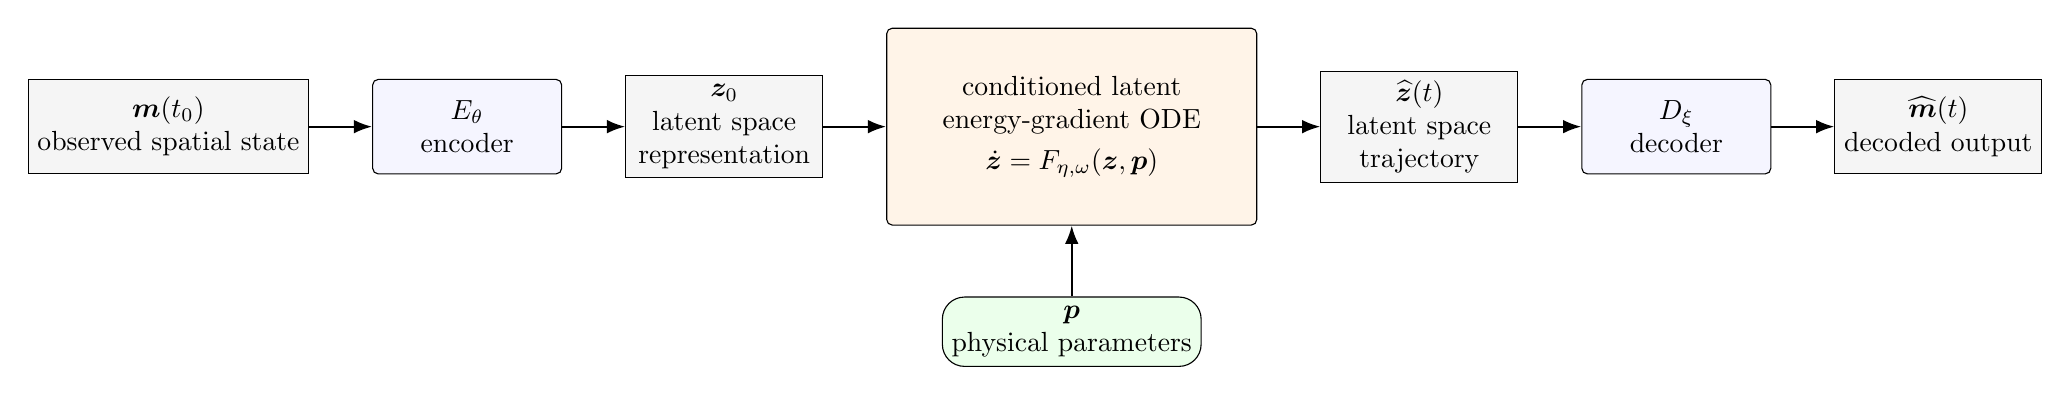
\begin{tikzpicture}[node distance=7mm and 8mm,>=Latex,
 block/.style={draw,rounded corners=2pt,align=center,minimum height=12mm,minimum width=24mm,fill=blue!4},
 state/.style={draw,align=center,minimum height=12mm,minimum width=25mm,fill=gray!8},
 ode/.style={draw,rounded corners=2pt,align=center,minimum height=25mm,minimum width=47mm,fill=orange!9},
 parameter/.style={draw,rounded corners=8pt,align=center,fill=green!8},arrow/.style={->,thick}]
\node[state] (m0) {$\m(t_0)$\\observed spatial state};
\node[block,right=of m0] (enc) {$\Eenc$\\encoder};
\node[state,right=of enc] (z0) {$\z_0$\\latent space \\representation};
\node[ode,right=of z0] (ode) {conditioned latent \\energy-gradient ODE\\[1mm]
$\dot\z=F_{\eta,\omega}(\z,\p)$};
\node[state,right=of ode] (zt) {$\zhat(t)$\\latent space \\trajectory};
\node[block,right=of zt] (dec) {$\Ddec$\\decoder};
\node[state,right=of dec] (mt) {$\widehat\m(t)$\\decoded output};
\node[parameter,below=9mm of ode] (p) {$\p$\\physical parameters};
\draw[arrow] (m0)--(enc); \draw[arrow] (enc)--(z0); \draw[arrow] (z0)--(ode);
\draw[arrow] (ode)--(zt); \draw[arrow] (zt)--(dec); \draw[arrow] (dec)--(mt); \draw[arrow] (p)--(ode);
\end{tikzpicture}}
\caption{Overall architecture. The encoder is evaluated at the initial state, the ODE advances the latent space representation, and the decoder supplies requested outputs. Physical parameters condition the latent energy-gradient ODE.}
\label{fig:architecture}
\end{figure}

\section{Latent energy-based dynamics}\label{sec:latent-dynamics}
\subsection{Scalar potential and gradient force}
Let the latent energy model $\Genergy:\mathcal Z\times\mathcal P\to\R$ be differentiable. Its first argument is the latent
state $\z\in\R^d$ and its second argument is the trajectory parameter
$\p\in\R^{n_p}$. We define the latent force
\begin{equation}
  \s(\z,\p)
  :=\nabla_{\z}\Genergy(\z,\p)
  \in\R^d.
  \label{eq:latent_force}
\end{equation}
The gradient is taken only with respect to $\z$ while $\p$ is fixed.

Nonlinearity in $\z$ is important for general trajectories. If $g(\z)=a^{\mathsf T}\z+b$, its gradient is constant and an autonomous model has constant velocity. If $g(\z)=\tfrac12\z^{\mathsf T}Q\z+a^{\mathsf T}\z+b$ with symmetric $Q$, its gradient is affine and the resulting vector field is affine. A deep scalar model permits both gradient and Hessian to vary with state. In \Cref{sec:results} we show that a combination of quadratic and deep scalar model is most effective.

\subsection{Conservative--dissipative split}
Let $\Jop,\Rop\in\R^{d\times d}$ satisfy
\begin{equation}
 \Jop^{\mathsf T}=-\Jop,\qquad \Rop^{\mathsf T}=\Rop,\qquad \Rop\succeq0.
 \label{eq:operator-conditions}
\end{equation}
The latent ODE in \Cref{fig:architecture} is
\begin{equation}
  \boxed{
  \dot\z(t)
  =F_{\eta,\omega}(\z(t),\p)
  =(\Jop-\Rop)\nabla_{\z}g_\eta(\z(t),\p).
  }
  \label{eq:latent-ode}
\end{equation}
Here $\dot\z=\mathrm d\z/\mathrm dt$. The operator $\Jop$ generates motion
that does not change $g_\eta$, whereas $-\Rop$ generates motion down its
gradient. The two terms use the same scalar potential but play distinct
dynamical roles.

The operators $\Jop, \Rop$ are constant with respect to $\z$ and $t$ in the present model.
They are nevertheless learned parameters. Their constancy is a deliberate
restriction and allow the latent dynamics to evolve in a fixed linear subspace of $\mathcal{Z}$ during inference. 
Nonlinear state dependence is assigned to the potential, while
the operators encode a simple global latent motion. 

\begin{proposition}[Autonomous latent-energy dissipation]
For fixed $\p$, a differentiable solution of \eqref{eq:latent-ode} satisfies
\begin{equation}
 \frac{\mathrm d}{\mathrm dt}\Genergy(\z(t),\p)=-\s^{\mathsf T}\Rop\s\leq0.
 \label{eq:dissipation}
\end{equation}
\end{proposition}
\begin{proof}
The chain rule and \eqref{eq:latent-ode} give
\begin{align}
 \frac{\mathrm d}{\mathrm dt}\Genergy(\z(t),\p)
 &=\s^{\mathsf T}\dot\z
 =(\s^{\mathsf T}\Jop\s-\s^{\mathsf T}\Rop\s).
\end{align}
Since $\Jop^{\mathsf T}=-\Jop$, a scalar $\s^{\mathsf T}\Jop\s$ equals its negative and vanishes. Positive semidefiniteness of $\Rop$ gives the result.
\end{proof}

The result is exact in continuous time and requires no dissipation penalty in
the training loss. It does not say that the observation-space trajectory
decreases a known physical energy. It says that the learned scalar
$g_\eta$ is a Lyapunov-like quantity for the learned autonomous latent flow.

If the parameter varies with time, $\p=\p(t)$, then
\begin{equation}
 \frac{\mathrm d}{\mathrm dt}\Genergy(\z(t),\p(t))=-\s^{\mathsf T}\Rop\s+\nabla_{\p}\Genergy(\z(t),\p(t))^{\mathsf T}\dot\p.
 \label{eq:nonautonomous-energy}
\end{equation}
The second term on the right hand side represents work associated with parameter variation. Therefore, monotonicity is guaranteed only if $\p$ is constant, or if this additional term is non-positive.

\begin{remark}
The autoencoder might or might not retain the spatial dimensions through global pooling. In our implementation we retained the spatial dimension. The  derivations also apply for general antisymmetric and semi-positive definite operators. For instance, if the spatial dimensions are kept and the latent operators are applied along the channel dimension. However, an important detail, is that if the spatial dimension is retained, one should also allow for energy transport within the spatial dimensions. Therefore, for the following deep energy model in \Cref{sec:results}, we use a convolutional layer with kernel width 3 as the first layer. It would also be possible to model the spatial energy transport with operators $\Jop$ and $\Rop$. However, imposing this property on the energy model is simpler, especially since we only used valid padding for all convolutional operations and doing both would be redundant.
\end{remark}

\subsection{Spectral properties of the operators}
The structural assumptions also constrain the spectra of the constant
operators. Although these spectra do not by themselves determine the nonlinear
dynamics, they are useful for verifying a trained model and further model analysis.

\begin{proposition}[Operator spectra]
Let $\Jop,\Rop\in\R^{d\times d}$ satisfy
$\Jop^{\mathsf T}=-\Jop$ and $\Rop\succeq0$, and define
$\Kop=\Jop-\Rop$. Then:
\begin{enumerate}[label=(\roman*)]
  \item every eigenvalue of $\Jop$ is purely imaginary or zero;
  \item every eigenvalue of $\Rop$ is real and nonnegative; and
  \item every eigenvalue $\lambda$ of $\Kop$ satisfies
        $\operatorname{Re}(\lambda)\leq0$.
\end{enumerate}
\label{prop:operator_spectra}
\end{proposition}

\begin{proof}
The first two statements are standard consequences of real antisymmetry and
real symmetric positive semidefiniteness. For the third, let
$\bm v\in\mathbb C^d\setminus\{\bm0\}$ satisfy
$\Kop\bm v=\lambda\bm v$, and let $\bm v^\ast$ denote its conjugate transpose.
Then
\begin{equation}
  \lambda
  =\frac{\bm v^\ast\Jop\bm v}{\bm v^\ast\bm v}
   -\frac{\bm v^\ast\Rop\bm v}{\bm v^\ast\bm v}.
\end{equation}
The first quotient is purely imaginary, while the second is real and
nonnegative. Therefore
\begin{equation}
  \operatorname{Re}(\lambda)
  =-\frac{\bm v^\ast\Rop\bm v}{\bm v^\ast\bm v}
  \leq0.
\end{equation}
\end{proof}
The eigen-decomposition of $\Jop$ and $\Rop$ help to analyze the importance of certain latent directions for the dynamics. Further, they are useful for rank estimation of a potential low-rank ansatz. They do not remove the coordinate and potential-scale ambiguities discussed later. 

\subsection{Conservative motion, dissipation, and equilibria}
If $\Rop=0$, velocity is orthogonal to the energy gradient and motion is tangent to energy level sets. If $\Jop=0$, the model is a generalized gradient flow. The combined field superposes these motions. Every critical point, $\s(\z_\star,\p)=0$, is an equilibrium. The converse need not hold: a nonzero gradient can lie in the nullspace of $\Kop$.

The dissipation rate vanishes when $\Rop\s=0$. The state can still move under $\Jop\s$. Hence, zero dissipation is not equivalent to equilibrium.

\begin{remark}
    The dissipation identity does not imply that every equilibrium is asymptotically stable. Stability also depends on the local energy shape, operator nullspaces, and their interaction. In our implementation we included a trainable regularizing term $\beta I$, with $\beta > 0$, to ensure full rank of $\Kop$, and hence, for an equilibrium $\z_\star$ it follows that $\s(\z_\star,\p)=0$. Especially for future applications for Gibbs free energy minimization tasks, this could be useful.
\end{remark}

\subsection{Nonlinear expressivity and local dynamics}
Constant matrices $\Jop$ and $\Rop$ do not make the model linear. For the vector field \eqref{eq:latent-ode} its state dependence is determined by the energy gradient only.

For a fixed parameter \(\p\), an affine energy produces a constant latent vector field. The encoder would therefore have to map each physical trajectory to straight-line motion with constant velocity in latent space. This is likely too restrictive to produce a useful latent representation of complex magnetization dynamics.

For a quadratic energy, $\nabla_{\z}g_{\mathrm{quad}}$ is affine in $\z$, and the resulting vector field is also affine. 
Although still restrictive, such dynamics may be sufficient for some applications. A convex quadratic energy additionally imposes a simple energy geometry and can therefore provide a useful inductive bias.

For a deep nonlinear energy, the gradient depends nonlinearly on $\z$, allowing the vector field to vary along a trajectory. This dependence is also visible in its Jacobian,
\begin{equation}
\frac{\partial F}{\partial\z}(\z,\p) = (\Jop-\Rop)\nabla_{\z}^{2}\Genergy(\z,\p),
\end{equation}
which is state dependent whenever the energy Hessian is state dependent.

The deep--quadratic model combines both contributions:
\begin{equation}
g_{\mathrm{deep\text{-}quad}}=g_{\mathrm{quad}}+g_{\mathrm{deep}},
\end{equation}
and hence
\begin{equation}
F_{\mathrm{deep\text{-}quad}}=(\Jop-\Rop)\nabla_{\z}g_{\mathrm{quad}} + (\Jop-\Rop)\nabla_{\z}g_{\mathrm{deep}}.
\end{equation}
The quadratic term provides an affine contribution, while the deep term provides a nonlinear correction. This decomposition is similar in spirit to the combination of linear and nonlinear terms in \cite{linot2023stabilized}, but here both terms are generated by energy gradients and retain the conservative--dissipative structure.

\subsection{Potential offset and scale}
For any parameter-dependent scalar $b(\p)$,
\begin{equation}\widetilde g(\z,\p)=\Genergy(\z,\p)+b(\p)\quad\Longrightarrow\quad \nabla_{\z}\widetilde g=\nabla_{\z}\Genergy.\end{equation}
Thus, the energy offset is unidentifiable. For any $a>0$,
\begin{equation}
 \widetilde g=a\Genergy,\qquad \widetilde\Jop=a^{-1}\Jop,\qquad \widetilde\Rop=a^{-1}\Rop
 \label{eq:scale-ambiguity}
\end{equation}
leaves the vector field unchanged. Trajectory supervision cannot fix an absolute energy or operator scale. Additional calibration or physical-energy supervision would be needed for physical interpretation. If such an additional calibration has practical benefits is an open question. 

\begin{remark}
A potential threat of energy supervision would be an increased stiffness of the latent dynamics, while a benefit could be better physical interpretation. However, we note that such supervision still does not guarantee that the learned effective field $\widetilde H_{\mathrm{eff}} = \frac{\partial \Genergy}{\partial \m} (\Ddec(\m))$ is a good approximation of the actual effective field unless snapshots are sampled at a sufficient temporal rate, and whether an increased temporal resolution increases the stiffness of the latent dynamics is another open question.
\end{remark}

\section{Learning from snapshot windows}
\subsection{Short windows extracted from long trajectories}

Let $\mathcal T$ denote the dataset of $M$ complete observed trajectories. During training, each trajectory is decomposed into contiguous windows of $k$ snapshots, yielding the windowed dataset
\begin{equation}
\mathcal T_k = \left\{\{(t_{\ell+i}^{(q)}, \m_{\ell+i}^{(q)}, \p^{(q)})\}_{i=0}^{k-1}\;:\;q=1,\ldots,M,\;\ell=0,\ldots,k_q-k
\right\}.
\label{eq:windowed-dataset}
\end{equation}

Windows may overlap, but complete physical trajectories are assigned to the training, validation, and test sets before window extraction. Hence, snapshots from the same trajectory cannot appear in different data partitions.

Each element of $\mathcal T_k$ is treated as an independent training sample. For a single window, the trajectory and window indices are omitted, and we write
\begin{equation}
\{\left(t_i,\m_i,\p\right)\}_{i=0}^{k-1}.
\end{equation}

The corresponding snapshots are encoded and give the latent reference states 
\begin{equation}
\z_i = \Eenc(\m_i), \qquad i=0,\ldots,k-1.
\end{equation}

The latent ODE~\eqref{eq:latent-ode} is integrated over $[t_0,t_{k-1}]$, with initial condition $\zhat(t_0) = \z_0$, and evaluated at the observation times $\zhat_i = \zhat(t_i)$ for $i=0,\ldots,k-1.$

The predicted latent states are compared to the actual latent reference states. Further, they are passed to the decoder which allows for comparison of the prediction in $\mathcal X$.
The numerical solver may use arbitrary internal time steps and only the solution values at the observation times are required for loss evaluation.

\subsection{Latent trajectory loss}
The latent trajectory loss compares the ODE solution with the encoded
observation sequence:
\begin{equation}
  \mathcal L_z
  =\frac{1}{(k-1)d}
   \sum_{i=1}^{k-1}
   \norm{\zhat_i-\z_i}_2^2.
  \label{eq:latent_loss}
\end{equation}
The initial index is omitted because $\zhat_0=\z_0$ by construction. This loss
encourages the encoder to produce coordinates whose evolution can be described
by the structured latent ODE. Because the targets $\z_i$ also depend on the
encoder parameters, $\mathcal L_z$ is coordinate dependent and can change
under a rescaling of the latent space.

\subsection{Decoded rollout loss and joint objective}
Accuracy in latent coordinates does not automatically imply accuracy after
decoding. We therefore compare the decoded integrated states directly with the
observations:
\begin{equation}
  \mathcal L_{\mathrm{roll}}
  =\frac{1}{3 k N}
   \sum_{i=0}^{k-1}
   \norm{\Ddec(\zhat_i)-\m_i}_2^2.
  \label{eq:rollout_loss}
\end{equation}
This term exposes the decoder to latent states reached by numerical
integration, not only to exact encoder outputs. It also anchors training to the
observable state rather than solely to a non-identifiable latent coordinate.
It is important to note that we do not omit the initial index for the rollout loss. This term is the exact reconstruction loss of the first state and notably improves training.

The full objective is given by
\begin{equation}
 \mathcal L(\Theta)=\lambda_z\mathcal L_z+\lambda_{\mathrm{roll}}\mathcal L_{\mathrm{roll}},\qquad \lambda_z,\lambda_{\mathrm{roll}}>0.
 \label{eq:objective}
\end{equation}
All parameters are optimized jointly. Gradients pass through the encoder targets, ODE solution, scalar gradient, operators, and decoder. The two losses counter simple degeneracies: the decoded term anchors the model to observations, while the latent term directly compares coordinate trajectories.

\section{Differentiation, integration, and scaling}

\subsection{Neural ODE viewpoint}
A neural ordinary differential equation specifies a parameterized vector field
$F_\Theta$ and defines predictions as the solution of an initial-value problem
\cite{chen2018neural},
\begin{equation}
  \dot\z(t)=F_\Theta(t,\z(t),\p),
  \qquad
  \z(t_0)=\z_0,
  \label{eq:generic_neural_ode}
\end{equation}
or, equivalently,
\begin{equation}
  \z(t)=\z_0+\int_{t_0}^{t}F_\Theta(\tau,\z(\tau),\p)\,\mathrm d\tau.
\end{equation}
Unlike a network with a fixed number of discrete layers, the requested output
times are handled by a numerical ODE solver, which may choose its own internal
steps. Training differentiates a loss through this numerical solution map. In
the present model, the vector field is $F_{\eta,\omega}$ from
\eqref{eq:latent-ode}, rather than an unrestricted neural network. The larger
training parameter set $\Theta=(\theta,\xi,\eta,\omega)$ additionally includes
the encoder and decoder parameters, although they are not part of the latent
right-hand side itself. While a generic neural ODE is certainly also a viable model for latent space integration, it imposes a less restrictive inductive bias compared to our energy based approach.


\subsection{Reverse-over-reverse differentiation}
At one right-hand-side evaluation, an inner reverse-mode derivative computes $\s=\nabla_{\z}\Genergy(\z,\p)$ and the operator produces $F=(\Jop - \Rop)\s$. Let $q_F$ be an incoming outer reverse-mode cotangent, defined by $\delta\mathcal L=q_F^{\mathsf T}\delta F$. Reverse differentiation through the operator gives
\begin{equation}
 q_s=(\Jop - \Rop)^{\mathsf T}q_F.
 \label{eq:gradient-cotangent}
\end{equation}
The outer derivative must propagate this sensitivity through the inner gradient in two directions. Its state contribution is the Hessian--vector product
\begin{equation}
 \left(\frac{\partial F}{\partial\z}\right)^{\mathsf T}q_F=\bm H_g(\z,\p)q_s,
 \label{eq:hvp}
\end{equation}
and its scalar-network parameter contribution is the mixed product
\begin{equation}
 \left(\frac{\partial F}{\partial\eta}\right)^{\mathsf T}q_F=
 \left(\frac{\partial}{\partial\eta}\nabla_{\z}\Genergy(\z,\p)\right)^{\mathsf T}q_s.
 \label{eq:mixed-product}
\end{equation}
Automatic differentiation evaluates these products without constructing a dense Hessian or mixed-derivative matrix. The calculation is reverse-over-reverse: an inner reverse pass constructs the field and an outer pass differentiates the loss through that construction and the numerical solve. 
Differentiating through adaptive solvers also requires care: continuous adjoints and direct discrete differentiation can produce different numerical gradients at finite tolerance \cite{gholami2019anode}.

\subsection{Continuous and discrete dissipation}
\eqref{eq:dissipation} concerns the exact continuous solution. A generic finite-tolerance integrator need not preserve monotonicity at every accepted step or saved output. A small numerical increase is distinct from violation of the analytic identity, which cannot occur when the operators satisfy
\eqref{eq:operator-conditions}. Solver selection and tolerances should therefore be reported as evaluation choices, not presented as part of the continuous-time guarantee.

\subsection{Computational scaling}
Let $C_g$ denote the cost of evaluating the scalar network and its gradient. One field evaluation costs approximately $C_g+\mathcal O(d^2)$ and operator storage is $\mathcal O(d^2)$ for dense operators. Structured rank-$r$ factorizations could reduce these contributions to $\mathcal O(dr)$ work and $\mathcal O(dr)$ storage if $r\ll d$. Antisymmetry and positive semidefiniteness can be retained through suitable factorizations, but the resulting rank restrictions may reduce expressivity and are not studied here. The decoder is evaluated at requested outputs rather than every internal ODE stage. This separation does not by itself establish a speed advantage: a meaningful comparison must include encoding, integration, decoding, and accuracy.

\begin{remark}
    If the latent space retains spatial dimensions the computational cost is $C_g+\mathcal O(|\mathcal S|d^2)$, where $|\mathcal S|$ denotes the number of spatial dimensions of the latent space.
\end{remark}

\section{Relation to structured dynamical models}
For canonical Hamiltonian dynamics, a fixed antisymmetric symplectic matrix acts on a Hamiltonian gradient. The antisymmetric term here has the same algebraic energy-preserving property, but the learned latent coordinates are not assumed canonical and the channel operator is learned. Pure gradient systems take the form $\dot\z=-M\nabla G(\z)$ with $M\succeq0$ and decrease $G$. The present field adds an antisymmetric component without changing the one-scalar dissipation identity.

Metriplectic and GENERIC formulations combine antisymmetric and symmetric brackets \cite{morrison1986paradigm,grmela1997dynamics}. Complete GENERIC formulations generally distinguish energy and entropy generators and impose additional degeneracy conditions. The one-scalar construction used here is simpler and should not be identified with those thermodynamic formalisms. Compared with an unrestricted latent neural ODE $\dot\z=f_\psi(\z,\p)$, the structured field occupies a smaller hypothesis class. It trades unrestricted vector-field flexibility for an exact continuous-time scalar-decrease property and explicit operator roles; whether that trade is beneficial requires empirical comparison.

\section{Numerical results}\label{sec:results}
We use the two applied-field directions of NIST $\mu$MAG Standard Problem~4 \cite{nist_sp4}: field~1 at $170^\circ$ and field~2 at $190^\circ$. Each comprises 200 uniformly spaced amplitudes: \SIrange{20.00}{29.95}{mT} for field~1 and \SIrange{30.00}{39.95}{mT} for field~2, at \SI{0.05}{mT} increments. Within these ranges, field1 exhibits comparatively smooth and regular dynamics, whereas field2 displays more complex trajectory variation.

The nominal trajectories at \SI{25}{mT} and \SI{36}{mT}, respectively, are held out as reference cases. The remaining 199 trajectories are split at trajectory level into 139 training trajectories $\mathcal{T}_{\mathrm{train}}$, 20 validation trajectories $\mathcal{T}_{\mathrm{val}}$, and 40 test trajectories $\mathcal{T}_{\mathrm{test}}$.

All trajectories begin from the same relaxed S-state and contain 101 snapshots from 0 to \SI{1}{ns}, inclusive, at \SI{0.01}{ns} intervals, on a $100\times25\times1$ grid with three magnetization components. Field amplitude is scaled to $[-1,1]$ using bounds fitted on the training set. This experiment concerns the stated grid and field directions only.

\subsection{Implementation and optimization}
The implemented encoder has channel widths $(16,32,64,128)$ and a matched transpose-convolution decoder. Its retained latent state has shape $4\times1\times1\times128$: four spatial sites with 128 channels each. All spatially nontrivial autoencoder and energy convolutions use \texttt{VALID} padding. Where a spatial extent is one, a numerically equivalent $1\times1\times1$ convolution is used when a larger \texttt{VALID} kernel is inapplicable. Hidden activations are GELUs.

\begin{table}[ht]
\centering\small
\caption{Implemented autoencoder. Counts include biases where present.}
\label{tab:architecture}
\begin{tabular}{llr}\toprule
Stage & output tensor & parameters\\\midrule
Input & $100\times25\times1\times3$ & 0\\
Encoder block 1 & $49\times11\times1\times16$ & 1,488\\
Encoder block 2 & $23\times4\times1\times32$ & 8,768\\
Encoder block 3 & $10\times1\times1\times64$ & 34,944\\
Encoder block 4 & $4\times1\times1\times128$ & 57,600\\
Latent $1\times1\times1$ convolution & $4\times1\times1\times128$ & 16,384\\
Decoder block 1 & $10\times1\times1\times128$ & 82,176\\
Decoder block 2 & $23\times4\times1\times64$ & 139,456\\
Decoder block 3 & $49\times11\times1\times32$ & 34,912\\
Decoder block 4 & $100\times25\times1\times16$ & 8,752\\
Reconstruction $1\times1\times1$ convolution & $100\times25\times1\times3$ & 48\\
\midrule Autoencoder total && 384,528\\\bottomrule
\end{tabular}
\end{table}

We compare three scalar-energy families. The quadratic model is
\begin{equation}
 g_{\mathrm{quad}}(\z,\p)=\tfrac12\norm{Q(\z)-c(\p)}_F^2,
\end{equation}
with a rank of 32. The VALID convolution gives $Q(\z)\in\mathbb R^{2\times1\times1\times32}$, while $c(\p)\in\mathbb R^{32}$ is broadcast over the two retained output sites; this model has 12,352 parameters. The deep model, denoted $g_{\mathrm{deep}}$, concatenates the physical parameters with the latent tensor broadcasted over the spatial sites. It then uses a spatial convolution followed by $1\times1\times1$ convolutions of widths $(32,32,16,1)$ with GELUs, sums the resulting scalar field, and applies softplus. It has 14,017 parameters. The deep--quadratic model is the direct additive combination
\begin{equation}
 g_{\mathrm{deep\text{-}quad}}(\z,\p)=g_{\mathrm{deep}}(\z,\p)+g_{\mathrm{quad}}(\z,\p),
\end{equation}
and has 26,369 parameters. The quadratic contribution supplies an affine term to the latent vector field, while the deep contribution permits state-dependent curvature. This rank-factorized quadratic energy is distinct from a low-rank channel-operator parameterization, which is not used.

The spatial convolutions in the energy models are structurally important because the channel operators act sitewise and do not themselves move information between retained sites. Both $Q$ in the quadratic model and the first layer of the deep model use a spatial kernel that mixes neighboring latent sites; the subsequent $1\times1\times1$ layers mix channels locally. Consequently, the gradient at one retained site can depend on neighboring latent states. The convolutions are therefore the model's direct route for representing cross-site coupling, including transport-like propagation or redistribution patterns in the latent dynamics. 

Each energy is paired with two vector-field families. The dissipative-only family uses $\dot\z_a=-\Rop\nabla_{\z_a}g$, whereas the antisymmetric--dissipative (A--D) family uses $\dot\z_a=(\Jop-\Rop)\nabla_{\z_a}g$. The channel operators are dense $128\times128$ matrices shared over the four sites: $\Jop=A-A^{\mathsf T}$ and $\Rop=B^{\mathsf T}B+\beta I$, with trainable positive $\beta$. Crossing the two fields with the quadratic, deep, and additive deep--quadratic energies gives the six compared models. The dissipative-only and A--D fields add 16,385 and 32,769 parameters, respectively. Complete-model counts, ordered as dissipative-only quadratic, deep, deep--quadratic, then A--D quadratic, deep, deep--quadratic, are 413,265, 414,930, 427,282, 429,649, 431,314, and 443,666.

We use a window size $k=5$, $\lambda_z=\lambda_{\mathrm{roll}}=1$, batch size 32, and 700 epochs. AdamW uses weight decay $10^{-4}$ and a learning rate that warms from $10^{-4}$ to $10^{-3}$ during the first 5\% of updates and then decays cosinusoidally to $10^{-5}$. 

Our implementation uses Diffrax \cite{kidger2021neural} with the explicit
Tsitouras $5(4)$ Runge--Kutta method (\texttt{Tsit5}). The relative tolerance is set to $10^{-3}$ and absolute tolerance to $10^{-5}$ for training and evaluation. The adaptive solver returns states at the snapshot times used by the loss even though its internal stages generally occur at different times.

Gradients are computed with Diffrax's \texttt{RecursiveCheckpointAdjoint}. This method differentiates the discrete solver computation by reverse-mode AD while retaining only selected primal states and recomputing others during the backward pass. Recursive checkpointing therefore trades additional computation for lower memory use. It should not be confused with a continuous backsolve adjoint that integrates a separate adjoint ODE backward in time. The checkpointed discrete adjoint differentiates the numerical trajectory actually produced by the chosen solver and tolerances. Checkpointing a discrete solve trades recomputation for storage, but it does not remove the products in \eqref{eq:hvp} and \eqref{eq:mixed-product}.

Evaluation uses one encoded initial state, no re-encoding of intermediate reference snapshots and no unit norm normalization. We use root mean square error (RMSE) as an error metric. Note that due to the unit norm constraint this also equals the relative RMSE (assuming the mean is not applied along the magnetization dimension). In addition, we report mean angular error (MAnE) as well as solver statistics.

The primary objective is to assess the overall model design and its applicability to this problem rather than to maximize predictive performance. Because the space of hyperparameters, architectural choices, and training algorithms is large, we use fixed configurations and do not perform systematic hyperparameter optimization. The reported results should therefore not be interpreted as estimates of the best attainable performance, and further tuning may yield substantial improvements.

\subsection{Joint vector-field and energy comparison}
Tables~\ref{tab:field1-comparison} and \ref{tab:field2-comparison} pool 40 held-out trajectories per field. The antisymmetric--dissipative deep--quadratic configuration has the smallest RMSE in this six-model, single-seed comparison: 0.0459 for field~1 and 0.2929 for field~2. For comparison, the reference solver (Tsit5 with relative tolerance $10^{-3}$ and absolute tolerance $10^{-5}$) requires \SI{0.349}{s} and \num{1034} steps for the field 1 case and \SI{0.330}{s} and \num{971} steps for the field 2 case on the same machine with single precision.

\begin{table}[ht]\centering\scriptsize
\caption{Field~1 comparison on 40 held-out trajectories (\SIrange{20.00}{29.95}{mT}, $170^\circ$). A--D denotes antisymmetric--dissipative and D dissipative-only. We report the RMSE for the windowed dataset $\mathcal{T}_\mathrm{test}^k$, and RMSE, MAnE, mean inference time (encoding, full rollout, and decoding) as well as required solver steps (accepted and rejected) for $\mathcal{T}_\mathrm{test}$.}\label{tab:field1-comparison}
\begin{tabular}{lrrrrrrrr}
\toprule
Model & parameters & RMSE for $\mathcal{T}_\mathrm{test}^k$ & RMSE & MAnE ($^\circ$) & s/trajectory & steps \\
\midrule
A--D quadratic & 429649 & 0.0070 & 0.3201 & 12.90 & 0.028 & 34.0 \\
A--D deep & 431314 & 0.0071 & 0.2063 & 6.71 & 0.047 & 40.4 \\
A--D deep--quadratic & 443666 & \textbf{0.0068} & \textbf{0.0459} & \textbf{1.68} & 0.073 & 50.2 \\
D quadratic & 413265 & 0.0091 & 0.7974 & 39.10 & 0.061 & 99.4 \\
D deep & 414930 & 0.0100 & 1.4309 & 64.75 & 0.040 & 28.9 \\
D deep--quadratic & 427282 & 0.0084 & 0.7922 & 38.26 & 0.099 & 70.2 \\
\bottomrule
\end{tabular}

\begin{table}[ht]\centering\scriptsize
\caption{As \Cref{tab:field1-comparison}, for field~2 (\SIrange{30.00}{39.95}{mT}, $190^\circ$).}\label{tab:field2-comparison}
\begin{tabular}{lrrrrrrrr}
\toprule
Model & parameters & RMSE for $\mathcal{T}_\mathrm{test}^k$ & RMSE & MAnE ($^\circ$) & s/trajectory & steps \\
\midrule
A--D quadratic & 429649 & \textbf{0.0411} & 0.7430 & 33.17 & 0.031 & 37.2 \\
A--D deep & 431314 & 0.0422 & 0.3363 & 12.23 & 0.053 & 46.1 \\
A--D deep--quadratic & 443666 & \textbf{0.0411} & \textbf{0.2929} & \textbf{9.47} & 0.094 & 47.4 \\
D quadratic & 413265 & 0.0442 & 1.3070 & 77.46 & 0.042 & 62.0 \\
D deep & 414930 & 0.0468 & 0.7632 & 31.49 & 0.040 & 30.0 \\
D deep--quadratic & 427282 & 0.0436 & 0.6678 & 29.05 & 0.095 & 70.3 \\
\bottomrule
\end{tabular}


\begin{figure}[ht]
\centering\includegraphics[width=.92\textwidth]{dissipative_failure_field1.pdf}
\caption{Uninterrupted dissipative-only deep--quadratic rollout at \SI{25}{mT}, $170^\circ$, on the $100\times25\times1$ grid. Solid curves are reference spatial means and dashed curves are decoded-model spatial means.}
\label{fig:dissipative-failure-field1}
\end{figure}

\begin{figure}[ht]
\centering\includegraphics[width=.92\textwidth]{dissipative_failure_field2.pdf}
\caption{As \Cref{fig:dissipative-failure-field1}, at \SI{36}{mT}, $190^\circ$.}
\label{fig:dissipative-failure-field2}
\end{figure}

It can be seen that a small error on the windowed dataset $\mathcal{T}_\mathrm{test}^k$ does not pose any strong guarantees for longer rollouts. 
The dissipative-only models have much smaller window errors than their uninterrupted-rollout errors, but do not reproduce the full rollouts in these two comparisons. This supports the usefulness of the antisymmetric term for these data and configurations. 

\Cref{fig:dissipative-failure-field1,fig:dissipative-failure-field2} show the uninterrupted dissipative-only deep--quadratic rollouts for the two reference fields. The comparison of predicted and reference mean magnetization illustrates how errors accumulate over a complete trajectory even when short-window errors remain small. Only dissipation of latent energy seems to be too restrictive to accurately learn the latent dynamics.

The quadratic energy model also has difficulties to reproduce the dynamics accurately and underfits the data even though the error is small on $\mathcal{T}_\mathrm{test}^k$.



\subsection{Reference trajectories, learned energy, and operator diagnostics}
\Cref{fig:best-rollout-field1,fig:best-rollout-field2} show the corresponding full reference-case rollouts for the antisymmetric--dissipative deep--quadratic models. Each figure presents the mean-magnetization trajectory together with its rollout error, the change in learned latent energy and the corresponding Gibbs energy of the reference. It can be seen that the latent energy does not qualitatively coincide with the Gibbs energy. The model performs quite good for field 1 and is able to capture the dynamics while the energy is decreasing along the trajectory. For the difficult field 2 case the model is still able to approximate the overall dynamics, however with a much larger error.

\begin{figure}[ht]
\centering\includegraphics[width=.92\textwidth]{best_rollout_field1.pdf}
\caption{Post-hoc test-leading antisymmetric--dissipative deep--quadratic rollout at \SI{25}{mT}, $170^\circ$: spatially averaged magnetization, RMSE, $g_\eta(t)-g_\eta(0)$ and scaled Gibbs energy of the reference solution. The rollout is evaluated on the $100\times25\times1$ grid with relative tolerance $10^{-3}$ and absolute tolerance $10^{-5}$. The learned latent energy does not correspond to the Gibbs energy.}\label{fig:best-rollout-field1}
\end{figure}

\begin{figure}[ht]
\centering\includegraphics[width=.92\textwidth]{best_rollout_field2.pdf}
\caption{As \Cref{fig:best-rollout-field1}, at \SI{36}{mT}, $190^\circ$.}\label{fig:best-rollout-field2}
\end{figure}

All saved learned-energy traces of the reported models were non-increasing. This observation is consistent with \eqref{eq:dissipation}.

The spatial structure of these rollouts is displayed in \Cref{fig:snapshots-field1,fig:snapshots-field2}. The angle maps compare the reference and decoded states at several times, while the error maps indicate vector differences.

\begin{figure}[ht]
\centering\includegraphics[width=.92\textwidth]{snapshots_field1.pdf}
\caption{Reference and decoded in-plane magnetization angle for the A--D deep--quadratic model at \SI{25}{mT}, $170^\circ$, on the $100\times25\times1$ grid. Both angle images use the common interval $[-\pi,\pi]$. The right column is the pointwise magnitude of the decoded-minus-reference magnetization vector, with one error scale shared across the four displayed times.}\label{fig:snapshots-field1}
\end{figure}

\begin{figure}[ht]\centering\includegraphics[width=.92\textwidth]{snapshots_field2.pdf}
\caption{As \Cref{fig:snapshots-field1}, at \SI{36}{mT}, $190^\circ$.}\label{fig:snapshots-field2}
\end{figure}


\begin{figure}[ht]
\centering\includegraphics[width=.82\textwidth]{operator_eigenvalues_field1.pdf}
\caption{Operator eigenvalues for the field~1 A--D deep--quadratic model. The left and middle panels histogram the imaginary parts of the $\Jop$ eigenvalues and real parts of the $\Rop$ eigenvalues; the right panel shows the complex spectrum of $\Kop=\Jop-\Rop$. The structure requires purely imaginary or zero eigenvalues for $\Jop$, nonnegative real eigenvalues for $\Rop$, and nonpositive real parts for eigenvalues of $\Kop$.}\label{fig:operator-eigenvalues-field1}
\end{figure}
\begin{figure}[ht]
\centering\includegraphics[width=.82\textwidth]{operator_eigenvalues_field2.pdf}
\caption{As \Cref{fig:operator-eigenvalues-field1}, for the field~2 A--D deep--quadratic model.}\label{fig:operator-eigenvalues-field2}
\end{figure}

\Cref{fig:operator-eigenvalues-field1,fig:operator-eigenvalues-field2} report the learned channel-operator spectra for the two selected models. 
These plots provide numerical diagnostics of the imposed antisymmetric and dissipative parameterizations. The antisymmetric operator exhibits a richer spectral structure, with conjugate eigenvalue pairs distributed over a broad interval of the imaginary axis. The substantially broader spectrum of the antisymmetric operator, compared with the dissipative eigenvalues clustered near zero, suggests that the antisymmetric component acts across a wider range of latent dynamical scales and likely plays a more important role in the learned evolution. For the parameter $\beta$, we find that the term is quite small after training: \num{3.766e-05} for field 1 and \num{1.364e-05} for field 2.


\begin{figure}[ht]
\centering\includegraphics[width=.92\textwidth]{training_field1.pdf}
\caption{Training and validation decoded-rollout and latent losses for the field~1 A--D deep--quadratic model.}\label{fig:training-field1}
\end{figure}
\begin{figure}[ht]
\centering\includegraphics[width=.92\textwidth]{training_field2.pdf}
\caption{As \Cref{fig:training-field1}, for the field~2 A--D deep--quadratic model.}\label{fig:training-field2}
\end{figure}
The optimization histories in \Cref{fig:training-field1,fig:training-field2} show the training and validation contributions used to fit the two selected models. For field 2, both training and validation losses remain comparatively high compared to the field 1 case. This could indicate underfitting. We also see a slight generalization gap and more data could help.

\subsection{Extrapolation beyond the training horizon}
The A--D deep and deep--quadratic models were extended to \SI{2}{ns} to further test generalization. The paired mean-magnetization trajectories and their errors are shown in \Cref{fig:extrapolation-field1,fig:extrapolation-field2}. The vertical marker separates the training horizon from the extrapolated interval and makes the subsequent error development visible for both energy models. 

For field 1, the deep–quadratic model remains close to the full-order reference throughout the \(\SI{2}{ns}\) interval and reproduces the qualitative magnetization evolution beyond the training horizon. In contrast, the deep model quickly departs from the reference and relaxes toward a spurious state. This result suggests that the quadratic contribution provides a useful inductive bias for preserving the relevant long-time dynamics in this case. For field 2, the deep-quadratic model still performs better than the deep model. It is closer to the reference, but the difference is less clear. The quadratic energy contribution provides an affine component of the latent vector field and is analogous to linear components considered for long-time neural-ODE forecasting \cite{linot2023stabilized}.

\begin{figure}[ht]\centering\includegraphics[width=.92\textwidth]{extrapolation_field1.pdf}
\caption{Paired \SI{2}{ns} rollout at \SI{25}{mT}, $170^\circ$. The upper panel overlays spatially averaged reference, A--D deep, and A--D deep--quadratic magnetization; color denotes component and line style denotes source. The lower panel shows RMSE for both learned models. The vertical marker denotes the \SI{1}{ns} training horizon. Both models encode exact copies of the same fresh full-order reference state.}\label{fig:extrapolation-field1}\end{figure}
\begin{figure}[ht]\centering\includegraphics[width=.92\textwidth]{extrapolation_field2.pdf}
\caption{As \Cref{fig:extrapolation-field1}, at \SI{36}{mT}, $190^\circ$.}\label{fig:extrapolation-field2}\end{figure}

\clearpage

\section{Limitations and prospective applications}
The experiments use only one grid and two distinct field directions. We do not perform any hyperparameter tuning and do not quantify optimization variability. The dissipation identity does not establish trajectory accuracy, physical-energy recovery, stability, or robustness outside the sampled family. 

Learning the solution trajectories over larger conditional parameter spaces requires exponentially more data. A promising idea from energy-based models is to employ a bounded replay buffer of positive supervised PDE transitions. An offline active reference-solver could be advanced by one output interval, with the resulting one-step transitions or short windows stored in the buffer. An instance would be replaced after reaching a predefined termination criterion. This stochastic approach could allow the training over large conditional spaces.
To test this, an natural extension of the training data in this work could include a second conditional parameter (field magnitude and field angle). Further, a spatial latent structure allows for arbitrary input dimension for the encoder. An interesting direction would be the training with different input shapes and testing spatial generalization of the model. 

Low-rank channel-operator parameterizations could drastically decrease the required parameter count for the latent vector field model. The presented operator spectra indicate that this low-rank structure is useful, but introducing rank restrictions requires a separate study.

In integrated sensing, a compact latent rollout could be useful if task-specific accuracy, latency, and robustness are demonstrated. When trajectories share an initial state, it only needs to be encoded once and only a terminal state could be decoded if intermediate fields are unnecessary. For observables, such as mean magnetization, a lightweight latent-to-observable head could replace the decoder completely. This could potentially result in a very lightweight model class.

\section{Conclusion}
We formulated a reduced order model coupling an autoencoder model to a conservative--dissipative energy-gradient ODE. Its continuous autonomous flow decreases the learned scalar latent energy while an antisymmetric operator allows for motion along the contour lines. We paired the vector field model with three different latent energy models, a deep, a quadratic, and a deep--quadratic model. These models were tested on two generated dataset for the NIST $\mu$MAG Standard Problem~4. One dataset for the field 1 case and one for the difficult field 2 case. The results give empirical evidence that the antisymmetric operator is a requirement to accurately learn a conditioned latent energy-gradient ODE for the dynamics. In paired post-hoc \SI{2}{ns} rollouts, for the field 1 case, the deep--quadratic model set a strong inductive bias and allowed for realistic generalization past the training horizon.\\

\textbf{Data.} The source code used to produce the results is publicly available on Zenodo \cite{ebm_2026_22281255}.

\newpage

\section*{Acknowledgment} 
This research was funded in whole or in part by the Austrian Science Fund (FWF) [10.55776/PAT7615923, 10.55776/P35413]. For the purpose of Open Access, the authors have applied a CC BY public copyright license to any Author Accepted Manuscript (AAM) version arising from this submission. The computations were partly achieved by using the Austrian Scientific Cluster (ASC) via the funded projects No. 71140, 71952 and 72862.

%\bibliographystyle{abbrv}
%\bibliography{references}

\begin{thebibliography}{10}

\bibitem{bashir2012head}
M.~Bashir, T.~Schrefl, J.~Dean, A.~Goncharov, G.~Hrkac, D.~Allwood, and D.~Suess.
\newblock Head and bit patterned media optimization at areal densities of 2.5 {T}bit/in2 and beyond.
\newblock {\em Journal of Magnetism and Magnetic Materials}, 324(3):269--275, 2012.

\bibitem{brown1963micromagnetics}
W.~F. Brown, Jr.
\newblock {\em Micromagnetics}.
\newblock Interscience Publishers, New York, 1963.

\bibitem{champion2019data}
K.~Champion, B.~Lusch, J.~N. Kutz, and S.~L. Brunton.
\newblock Data-driven discovery of coordinates and governing equations.
\newblock {\em Proceedings of the National Academy of Sciences}, 116(45):22445--22451, 2019.

\bibitem{chen2018neural}
R.~T. Chen, Y.~Rubanova, J.~Bettencourt, and D.~K. Duvenaud.
\newblock Neural ordinary differential equations.
\newblock {\em Advances in neural information processing systems}, 31, 2018.

\bibitem{du2019implicit}
Y.~Du and I.~Mordatch.
\newblock Implicit generation and modeling with energy based models.
\newblock {\em Advances in neural information processing systems}, 32, 2019.

\bibitem{exl2021prediction}
L.~Exl, N.~J. Mauser, S.~Schaffer, T.~Schrefl, and D.~Suess.
\newblock Prediction of magnetization dynamics in a reduced dimensional feature space setting utilizing a low-rank kernel method.
\newblock {\em Journal of Computational Physics}, 444:110586, 2021.

\bibitem{fischbacher2018micromagnetics}
J.~Fischbacher, A.~Kovacs, M.~Gusenbauer, H.~Oezelt, L.~Exl, S.~Bance, and T.~Schrefl.
\newblock Micromagnetics of rare-earth efficient permanent magnets.
\newblock {\em Journal of Physics D: Applied Physics}, 51(19):193002, 2018.

\bibitem{gholami2019anode}
A.~Gholami, K.~Keutzer, and G.~Biros.
\newblock Anode: Unconditionally accurate memory-efficient gradients for neural odes.
\newblock {\em arXiv preprint arXiv:1902.10298}, 2019.

\bibitem{gilbert2004phenomenological}
T.~L. Gilbert.
\newblock A phenomenological theory of damping in ferromagnetic materials.
\newblock {\em IEEE transactions on magnetics}, 40(6):3443--3449, 2004.

\bibitem{greydanus2019hamiltonian}
S.~Greydanus, M.~Dzamba, and J.~Yosinski.
\newblock {H}amiltonian neural networks.
\newblock {\em Advances in neural information processing systems}, 32, 2019.

\bibitem{grmela1997dynamics}
M.~Grmela and H.~C. {\"O}ttinger.
\newblock Dynamics and thermodynamics of complex fluids. i. development of a general formalism.
\newblock {\em Physical Review E}, 56(6):6620, 1997.

\bibitem{hernandez2023port}
Q.~Hern{\'a}ndez, A.~Bad{\'\i}as, F.~Chinesta, and E.~Cueto.
\newblock Port-metriplectic neural networks: thermodynamics-informed machine learning of complex physical systems.
\newblock {\em Computational Mechanics}, 72(3):553--561, 2023.

\bibitem{hinton2002training}
G.~E. Hinton.
\newblock Training products of experts by minimizing contrastive divergence.
\newblock {\em Neural computation}, 14(8):1771--1800, 2002.

\bibitem{kidger2021neural}
P.~Kidger.
\newblock {\em On Neural Differential Equations}.
\newblock PhD thesis, University of Oxford, 2021.

\bibitem{kovacs2020computational}
A.~Kovacs, J.~Fischbacher, M.~Gusenbauer, H.~Oezelt, H.~C. Herper, O.~Y. Vekilova, P.~Nieves, S.~Arapan, and T.~Schrefl.
\newblock Computational design of rare-earth reduced permanent magnets.
\newblock {\em Engineering}, 6(2):148--153, 2020.

\bibitem{kovacs2019learning}
A.~Kovacs, J.~Fischbacher, H.~Oezelt, M.~Gusenbauer, L.~Exl, F.~Bruckner, D.~Suess, and T.~Schrefl.
\newblock Learning magnetization dynamics.
\newblock {\em Journal of Magnetism and Magnetic Materials}, 491:165548, 2019.

\bibitem{lee2020model}
K.~Lee and K.~T. Carlberg.
\newblock Model reduction of dynamical systems on nonlinear manifolds using deep convolutional autoencoders.
\newblock {\em Journal of Computational Physics}, 404:108973, 2020.

\bibitem{linot2023stabilized}
A.~J. Linot, J.~W. Burby, Q.~Tang, P.~Balaprakash, M.~D. Graham, and R.~Maulik.
\newblock Stabilized neural ordinary differential equations for long-time forecasting of dynamical systems.
\newblock {\em Journal of Computational Physics}, 474:111838, 2023.

\bibitem{morrison1986paradigm}
P.~J. Morrison.
\newblock A paradigm for joined {H}amiltonian and dissipative systems.
\newblock {\em Physica D: Nonlinear Phenomena}, 18(1-3):410--419, 1986.

\bibitem{nist_sp4}
{NIST Micromagnetic Modeling Activity Group}.
\newblock \url{https://www.ctcms.nist.gov/~rdm/std4/spec4.html}. Accessed 31 July 2026.

\bibitem{rubanova2019latent}
Y.~Rubanova, R.~T. Chen, and D.~K. Duvenaud.
\newblock Latent ordinary differential equations for irregularly-sampled time series.
\newblock {\em Advances in neural information processing systems}, 32, 2019.

\bibitem{ebm_2026_22281255}
S.~Schaffer and L.~Exl.
\newblock ebm\_llg, Sept. 2026.
\newblock \url{https://doi.org/10.5281/zenodo.22281255}.

\bibitem{schaffer2021machine}
S.~Schaffer, N.~J. Mauser, T.~Schrefl, D.~Suess, and L.~Exl.
\newblock Machine learning methods for the prediction of micromagnetic magnetization dynamics.
\newblock {\em IEEE Transactions on Magnetics}, 58(2):1--6, 2021.

\bibitem{suess2018topologically}
D.~Suess, A.~Bachleitner-Hofmann, A.~Satz, H.~Weitensfelder, C.~Vogler, F.~Bruckner, C.~Abert, K.~Pr{\"u}gl, J.~Zimmer, C.~Huber, et~al.
\newblock Topologically protected vortex structures for low-noise magnetic sensors with high linear range.
\newblock {\em Nature Electronics}, 1(6):362--370, 2018.

\bibitem{tieleman2008training}
T.~Tieleman.
\newblock Training restricted {B}oltzmann machines using approximations to the likelihood gradient.
\newblock In {\em Proceedings of the 25th international conference on Machine learning}, pages 1064--1071, 2008.

\end{thebibliography}


\end{document}
